\documentclass[11pt,a4paper]{article}
\usepackage[a4paper, total={6.5in, 10.5in}]{geometry}
\usepackage{graphicx}
\usepackage{caption}
\usepackage{subcaption}
\usepackage{cite}
 
\begin{document}
\title{Review of Passive Wireless Sensors}
\author{Jakub M. Szypicyn}
\date{November 2017}
\maketitle
\tableofcontents
\pagebreak
\section{Introduction}

Passive wireless sensors (PWS) are a type of instrumentation that requires no local power source or leads to works. The principle of operation is such that incident inductive or RF power is harvested, modulated and reflected back. Harvesting requires either a coil if the power is transmitted inductively or an antenna in the case of RF. Modulation of the incoming waveform then takes place. It is at this point that the sensed information is being uniquely encoded in the signal. The power is then retransmitted back to the interrogator.

Passive wireless sensing is not exactly a brand new invention. Radar for example can be regarded as a system utilising the principle of PWS. Though it isn't a sensor \textit{per se}, it works by firing a pulse of energy, which upon interaction with physical objects is reflected back. Thus this system can be regarded as passive wireless detector.

However, several weeks before the end of the World War II Soviet inventor Léon Theremin came up with what was later called as "The Thing" - a passive wireless listening device or simply a bug. Notably, "The Thing" was used to spy on the United States Ambassador to the Soviet Union W. Averell Harriman during the Cold War. 

"The Thing" operated by harvesting RF power using a quarter-wavelength antenna. The sensing circuit consisted of a resonant cavity, in which capacitor acted as a modulating elements. The sound waves would set the capacitor's membrane into vibration. The amplitude modulated (AM) signal was retransmitted and demodulated at the reader side. This device is considered as a predecessor to modern RFID technology\cite{thing}.

The passive wireless sensors have therefore come a long way since 1945. The types of application have varied throughout this time. In 1973 first true tagging system with intention of using it as a road toll system had been patented \cite{toll}.

Nowadays PWSs are used whenever the measurand is not easily accessible, wires cannot be connected, low production cost is required, simple electronic circuits are preferred or the device is meant to operate in extreme environments. The following section discusses modern age technologies and solutions, which enable passive wireless sensing.

\section{Current Technologies}

\subsection{LC-Resonant Tank}

By far the most common implementation of a passive wireless sensor is that involving a resonant structure using lumped elements. The basic principle of such sensor is quite straight forward. One of the elements of the resonant structure is exposed to the measurand. As the environment around for example the capacitor varies, its capacitance varies too, to reflect the sensed changes. Depending on the measured quantity the variation may be linear, otherwise additional processing techniques are employed at the read-out stage.

Depending on the method of exposing one or more elements of the circuit to the measurand, both capacitor or inductor can play the role of a sensor. The following publications propose using capacitors as direct sensors of the environment.

Qiulin \textit{et al.} \cite{harsh} propose using a dual LC resonant circuit to simultaneously measure pressure and temperature. Both LC circuits utilise capacitors to measure the quantities. In order to sense pressure they have employed a cavity capacitor, whereas to sense temperature LTCC \cite{LTCC} was used to fill the gap between electrodes. The model is shown in Figure \ref{fig:harsh1}.

\begin{figure}[h]
\centering
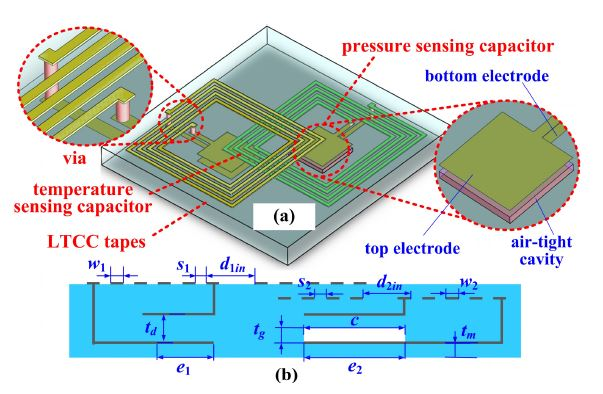
\includegraphics[width=0.75\textwidth]{harsh1.JPG}
\caption{Schematic of the sensor. (a) Persective view and (b) cross-sectional view. \cite{harsh}\label{fig:harsh1}}
\end{figure}

The resonant frequencies can be accurately approximated as

\begin{equation}
f_t = \frac{1}{2\pi \sqrt{L_1C_1}}, \quad f_p = \frac{1}{2\pi \sqrt{L_2C_2}}
\end{equation}

where $f_t$ and $f_p$ are the resonant frequencies of the temperature and pressure sensing circuits respectively. In this model it is clear that by applying pressure which is normal the the largest surface in Figure \ref{fig:harsh1} (a), the air cavity height will vary, thus changing the capacitance.

Equivalently, LTCC filled capacitor is used to sense temperature, as the dielectric properties of the material will be affected by the change in temperature. LTCC material is assumed incompressible and thus it is predicted that the temperature sensor will be independent of the applied pressure. However the research group has realised that there is some dependency between pressure measurement and the temperature and therefore they propose to employ a post processing technique to compensate for the temperature in pressure measurements.

All in all, the have found that their sensor is functional in harsh environments up to 673 K. Moreover the temperature and pressure sensitivities are reported to reach 8.15 kHz/K and 1.96 MHz/Bar, respectively.

Similarly to the previous group Ren \textit{et al.} \cite{graphene} propose to use an LC tank where the capacitor is sensitive to temperature. Rather than using a parallel plate capacitor they decided to employ an interdigital capacitor (IDC) due to preferred fabrication techniques.

The space between fingers of the IDC has been filled with thin layer of graphene oxide, whose electrical properties has been found to vary with electric field, temperature or light. It is the temperature dependency that they have exploited. This is a very similar implementation of a sensor as presented by Quilin \textit{et al.} Figure \ref{fig:IDC} shows the fabrication technique used to manufacture this device.

\begin{figure}[h]
\centering
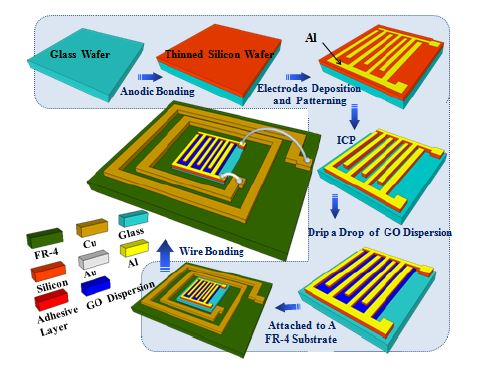
\includegraphics[width=0.5\textwidth]{graphene1.JPG}
\caption{Fabrication process of the interdigital capacitive temperature sensor. \cite{graphene}\label{fig:IDC}}
\end{figure}

The graphene-oxide based device has been tested for temperatures ranging from 233 K to 333 K. It has been found that the sensor has two regions of linearity with different sensitivities. From 233 K to 273 K the sensitivity was measured to be 59.3 kHz/K and from 283 K to 333 K it is 46.1 kHz/K. These values are a factor of 6-7.5 higher than those reported by Quilin \textit{et al.}

The same structure as above, only without the graphene  has been employed by Jia \textit{et al.} \cite{IDC} to measure strain. Since the capacitance of the IDC depends on the spacing between its fingers, strain along one of the axis will result in change of the resonant frequency of the device. 

It is not inconceivable to imagine other similar structures that use the change of the dimensions of either capacitor or inductor to measure some physical phenomena. For instance, corrosion can be measured by exposing a capacitor to the metal surface. As corrosion occurs the capacitor will be filled with external substance - water or oxide, thus changing the dielectric property of the capacitor \cite{corrosion}.

Though this approach is fairly simple, the above research publications only interrogate the sensors inductively. This means that the maximum achieved distance is only a few centimetres for a reasonable input power. It should in theory be possible to interrogate the same devices with addition of an antenna using RF power. Lumped elements should in theory be behaving predictably up to around 20 GHz. This should therefore allow to significantly extend the operational range at the cost of increased size due to the requirement of having an antenna.

\subsection{Frequency Selective Surfaces}

Yasri \textit{et al.} \cite{corrosion2} proposed using microstrip resonant stubs to sense corrosion. The idea is somewhat basic. By exposing the resonant stub to the atmospheric conditions experienced by the object of interest, they were able to determine the shift in resonant frequency. As the microstrip stub corrodes its functional length decreases hence increasing the resonant frequency. The idea is presented in Figure \ref{fig:stub}.

\begin{figure}[h]
\centering
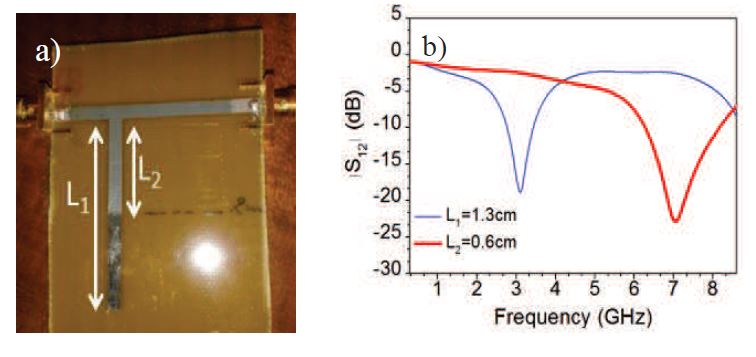
\includegraphics[width=0.75\textwidth]{stub.JPG}
\caption{The stub resonantor after corrosion (a) and the resonance frequency shift induced by the corrosion process (b).\cite{corrosion2}\label{fig:stub}}
\end{figure}

The challenge with using the above method is to provide realistic estimation of the corrosion taking place on the surface of the actual object rather than of the microstrip.

There has been some interest in using antenna's as direct sensors of strain and cracking. The three following publications focus on changing the geometry of the antenna and thus changing its resonant frequency.

Firstly, Yi \textit{et al.} \cite{array} propose using a folded-patch antenna. Their system utilises a backscattering mechanism and employs a cheap RFID chip in order to allow more than one sensor to be interrogated simultaneously. The chip is powered directly by the incoming RF radiation. The sensor design is shown in Figure \ref{fig:folded}.

\begin{figure}[h]
\centering
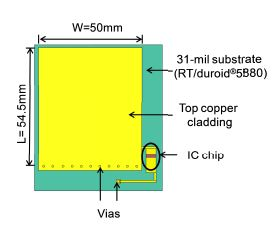
\includegraphics[width=0.375\textwidth]{folded.JPG}
\caption{RFID tag as wireless starin sensor - design drawing.\cite{array}\label{fig:folded}}
\end{figure}

If the incident power is above certain threshold power then the RFID tag will be activated and the sensor will reflect back its ID. The strain is measured by tracking the resonant frequency of the folded-patch antenna. Its zero-strain resonance can be estimated as

\begin{equation}
f_0 = \frac{c}{4(L+L')\sqrt{\epsilon _r}}
\end{equation}

where \textit{c} is the speed of light in vacuum, \textit{L} is the physical length of the top copper cladding, \textit{L'} is the additional electrical length due to fringing effects and $\epsilon _r$ is the relative dielectric permittivity of the substrate. When the antenna experiences longitudinal strain of $\epsilon$ its resonant frequency changes in the following manner

\begin{equation}
f_{\epsilon} = \frac{f_0}{1+\epsilon}
\end{equation}

Though this is a non-linear relationship, for small strains the above equation can be approximated as

\begin{equation}
f_{\epsilon} = f_0(1-\epsilon+\epsilon ^2-\epsilon ^3 ... ) \simeq f_0(1-\epsilon)
\end{equation}

which is very much linear.

Similarly to the previous study Tata \textit{et al.} \cite{patch} exploited a patch antenna to detect strain. As opposed to Yi \textit{et al.} this research group took advantage of the 2D structure of the antenna. Namely, the realised that a rectangular patch antenna will have two dominant resonant frequencies  - one for each dimension. The key idea is to provide incident power that is polarised in a way that enables excitation of the two modes.

In the paper they did not test the sensor wirelessly, but provided the input through a microstrip line. However as a proof of concept they showed that the two propagation modes TM$_{10}$ and TM$_{01}$ are sensitive enough to detect changes in strain.

In a paper \cite{horn} published by the same research group they propose to use a horn antenna in order to provide the incident radiation with the specified polarisation. It can be seen how this can cause problems when deployed. Any relative rotation of patch antenna and horn antenna will decrease the transmitted power and hence decrease the maximum operational distance.

Figure \ref{fig:patch} shows the wireless and wired sensors designs.

\begin{figure}[h]
\centering
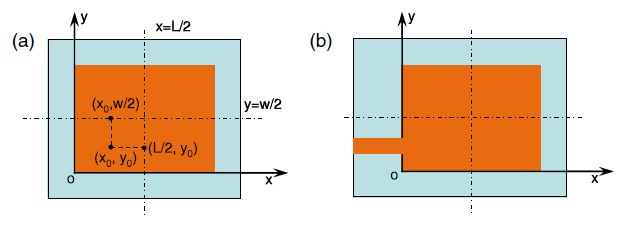
\includegraphics[width=0.75\textwidth]{patch.JPG}
\caption{Antenna feeding (a) 50 $\Omega$ impedance matching; (b) microstrip feed line.\cite{horn}\label{fig:patch}}
\end{figure}

\subsection{Other Resonant Structures}

There is a plethora of possible utilisations of resonant structures. In this section just one example will be presented as the general operation principle is shared by all resonant structures, i.e. either inductor or capacitor in the equivalent circuit model is used for sensing.

Zhao \textit{et al.} in \cite{evamode}  present a radio frequency evanescent-mode cavity resonator. The structure is made up of a cavity with a centre post. The resonant frequency of the structure is determined by the capacitance formed between the centre post and the top membrane of the cavity. In the paper they apply this idea to sense air flow. By attaching a deflection needle to the top of the membrane, as the air moves the needle, it inevitably increases or decreases the distance from the top membrane to the centre post. The cross-sectional view of the structure is shown in Figure \ref{fig:eva}.

\begin{figure}[h]
\centering
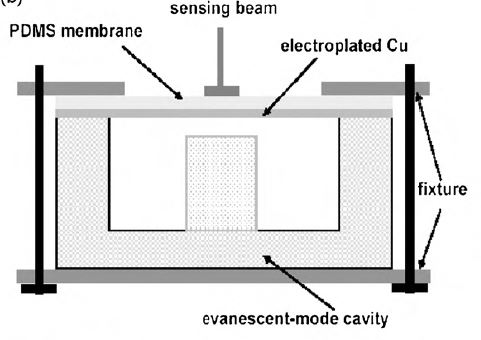
\includegraphics[width=0.5\textwidth]{cavity.JPG}
\caption{Cross-sectional view of the airflow sensor unit. \cite{evamode}\label{fig:eva}}
\end{figure}

The energy is radiated inside the cavity through a coplanar waveguide (CPW). The same CPW is then used to guide the resonant signal back to the antenna. The resonant frequency of the cavity can be approximated using the standard equation

\begin{equation}
f_0 \simeq \frac{1}{2\pi \sqrt{L C_{post}}}\textrm{,}
\end{equation}

where $L$ is the equivalent inductance due to surface current and $C_{post}$ is the capacitance formed between the post and top membrane. It should be noted that this approximation holds only when $C_{post}$  is the dominant capacitance in the structure, i.e. when the gap between the post and top membrane is much smaller than the dimensions of the cavity. It therefore  has been shown that the resonant frequency depends on the deflection angle as

\begin{equation}
f_r = f_0\sqrt{\frac{C}{C'}} = \left(\frac{d}{2r\theta}\textrm{ln}\left(\frac{(d/r)+\theta}{(d/r)-\theta}\right)\right)^{-\frac{1}{2}}\textrm{,}
\end{equation}

where $C$ is the nominal, or zero angle deflection, capacitance of the structure, $C'$ is the new capacitance, $d$ is the mean gap, $r$ is the radius of the capacitive post and $\theta$ is the defelction angle.

\subsection{Intermodulation Communication Principle}

This area of passive wireless sensors has been only researched by Professor Ville Viikari of Aalto University in Helsinki. In a paper written by Viikari \textit{et al.}\cite{imc_review} three techniques of achieving intermodulation communication principle (ICP) are described.

In short ICP relies on two signals at slightly different frequencies - \textit{f}$_1$ and \textit{f}$_2$ being received by the sensor. The sensor is some passive fashion will then mix the signals together. The modulated signal which depends on some physical phenomenon or phenomena will mix back with the incident waves and re-radiate a modulated signal.

In general mixers are constructed using transistors, i.e. these are active devices. However since the power budget is limited another method of mixing is sought after. Viikari discusses three methods - MEMS, electrically non-linear elements and low-frequency resonant circuits.

Beginning with MEMS, the receiving antenna is directly coupled to a capacitive MEMS resonator. The mechanical resonator will develop voltages at both frequencies. Howeve due to its non-linearity there will also be all the harmonic frequencies of type \textit{nf}$_1$ $\pm$ \textit{mf}$_2$. The capacitance of the resonator will be modulated by the mechanical vibrations, hence the reflection coefficient will vary with time. The outgoing refelction will be at frequencies equal to \textit{f}$_1$ $\pm$ \textit{f}$_{res}$ and \textit{f}$_2$ $\pm$ \textit{f}$_{res}$. In a case when the resonant frequency is the difference of the two incoming frequencies the intermodulation signals being re-radiated are 2\textit{f}$_1$ $-$ \textit{f}$_2$ and 2\textit{f}$_2$ $-$ \textit{f}$_1$. Furthermore it has been found that the voltage at the intermodulation frequency can be estimated as follows \cite{rfidMEMS}

\begin{equation}
V_{2f_2-f_1} \simeq \frac{\omega_m^2}{\Delta \omega^2 \left(1+\left( \frac{Q_m \left(\Delta \omega^2 - \omega_m^2 \right)}{\Delta \omega \omega_m} \right)^2 \right)}
\end{equation}

where $\Delta \omega = 2\pi (f_2-f_1)$, $\omega_m$ is the angular frequency of the resonator and $Q_m$ is its quality factor. As long as the MEMS' resonance frequency or the quality factor are dependent on the measurand the the device can act as a sensor. The problem with utilising this sensor is that its cut-off frequency is around 10 MHz. It is worth noting that in the above equation the generated voltage reaches unity when the resonance frequency is equal to the difference of the interrogation frequencies. The sensor must therefore not operate at the resonance frequency of the MEMS otherwise quality factor will not be sensed. Similarly, if the sensor utilises the resonant frequency of MEMS as sensing mechanism then it is ideal that the quality factor is reasonably large, however not as large as to decrease the dynamic range of the sensor. The higher the quality factor the sharper the roll off, thus the sensing capability decreases as there isn't enough retransmitted power. The plot of the voltage as a function of quality factor and MEMS resonant frequency is shown in Figure \ref{fig:vol}.


\begin{figure}[h]
\centering
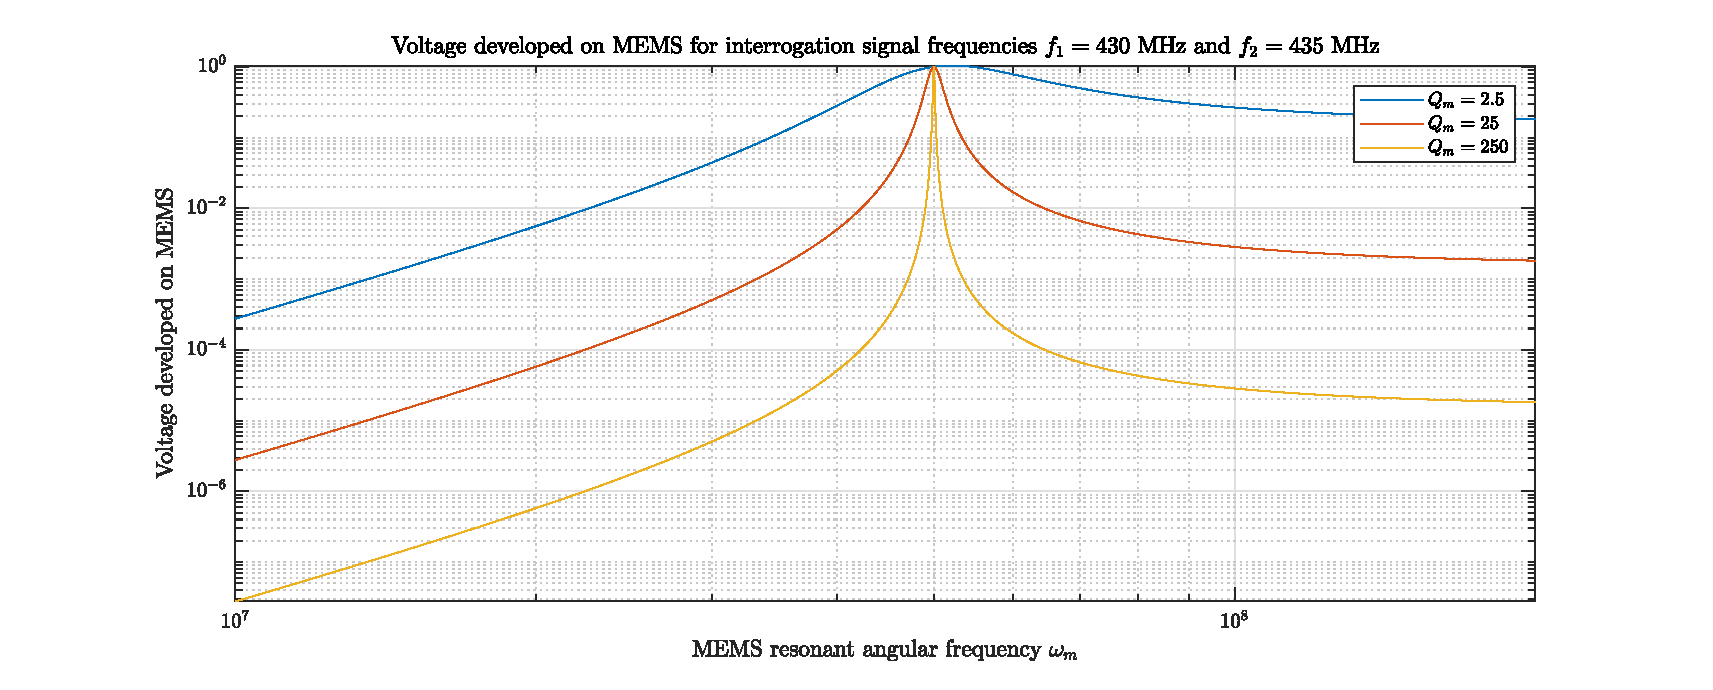
\includegraphics[width=1\textwidth]{voltage.eps}
\caption{Volatge developed on MEMS structure for varying resonant frequencies and quality factors.\label{fig:vol}}
\end{figure}

Viikari then discusses sensors based on electrically non-linear elements. This method has in fact been used by his research group \cite{icp1,icp2,icp3,icp4}. In short the same outcome as in using MEMS is achieved by employing electrically non-linear element such as a diode or micro-bolometer. More specifically he lists photo-diodes and varactor-diodes. Their non-linear behaviour and its non-idealities allow for signal mixing. It is found that the voltage at intermodulation frequency can be estimated as

\begin{equation}
V_{2f_2-f_1} \simeq Q^4(1 - |\Gamma|)^4
\end{equation}

where $\Gamma$ represents the reflection coefficient between the antenna and the varactor. The relationship between retransmitted power and either the reflection coefficient is straightforward. It is has been found by Viikari that the reflection coefficient is affected by the changes in temperature thus granting the device its sensing capabilities.

Finally, low frequency resonant circuits are proposed as means of mixing signals. It is said that utilising a single element for mixing and sensing can lead to unwanted behaviour. First of all, microwave mixing using these passive techniques is found to be inefficient. Additionally, it is difficult to realise a mixer as an efficient and accurate sensor. Lastly, the antenna impedance changes when it is placed in close proximity to a dielectric or conductive material. As such the reflection coefficient changes making the sensor virtually unusable. More sophisticated techniques are required to mix and and sense separately.

In general this sort of circuit would use an antenna coupled to a high pass filter which then feeds a mixing element. The mixing element is then connected to a low pass filter to extract the modulation components of interest. Finally, the low pass filter is loaded with a resonant circuit which employs a sensing element such as a capacitor. An equivalent circuit is shown in Figure \ref{fig:lowf}.

\begin{figure}[h]
\centering
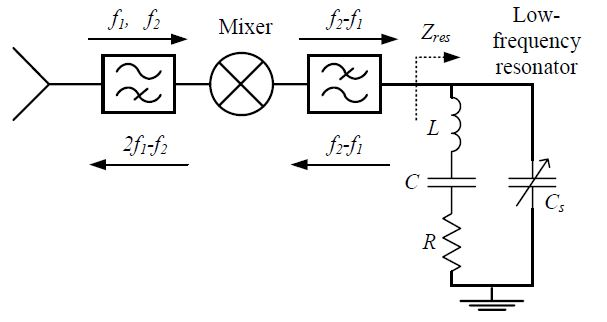
\includegraphics[width=0.5\textwidth]{low_f.JPG}
\caption{Simplified equivalent circuit of the intermodulation sensor based on a low-frequency resonator. \cite{rfidMEMS}\label{fig:lowf}}
\end{figure}

Due to two stage mixing process the voltage and thus the retransmitted power depends on the impedance of the resonator at the difference frequency as

\begin{equation}
V_{2f_2-f_1} \simeq A + BZ_{res}(f_{\Delta})
\end{equation}

where A and B are complex numbers independent of the difference frequency. It is therefore clear that modulation in the impedance of the resonant structure will shift the power level of the backscattered signal.

\subsection{Surface Acoustic Waves}

Surface acoustic wave (SAW) devices are known to work as simple RFID tags, but also as sensors of humidity, temperature, pressure, biologial and chemical reactions, strain or electric field variation. The surface wave also known as Rayleigh wave \cite{rayleigh} as the name suggests travels along the surface of the material and only penetrates the material roughly one wavelength deep. Hence all of the incoming RF energy can be efficiently transduced into useful mechanical energy, provided the means of transducing are efficient. 

To convert the RF signal into an elastic wave an interdigital transducer (IDT) deposited on the surface of a piezoelectric material is used. The elastic wave then propagates through the material. At this point we can distinguish two types of devices - single and double port devices.

In single port devices the same antenna and the same IDT are used to for the input and output. Analogically, double port devices use a pair of each. Most of the literature focuses on single port devices and as such all of the attention shall be given to them.

The properties of elastic waves strongly depend on the geometry of the material, shape of IDTs and the material deposited on the piezoelectric substrate \cite{SAWapps}. The main sensing paramater in SAW devices is the delay time of the wave. Firstly, an elastic wave travels three orders of magnitude slower than its electromagnetic counterpart. Secondly, the actual delay is a function of material length and wave velocity. 

\begin{equation}
T_d = \frac{L}{v_{SAW}}
\end{equation}

where $T_d$ is time delay, $L$ is path length and $v_{SAW}$ is the phase velocity. Both $L$ and $v_{SAW}$ are known to vary with the parameters listed earlier, e.g. strain. In single port devices the input signal will be converted into SAW. The elestic wave will then propagate through the surface of the material. In order to determine the time delay of the wave minimum of two reflectors are deposited in the path of the SAW. The wave will then partially be reflected by each of those structures and the signal will be backscattered to the receiver. A representation of that mechanism is shown in Figure \ref{fig:SAWbasic}. Hence by measuring the time between consecutive reflections at the read-out stage it is possible to resolve the measurand.

\begin{figure}[h]
\centering
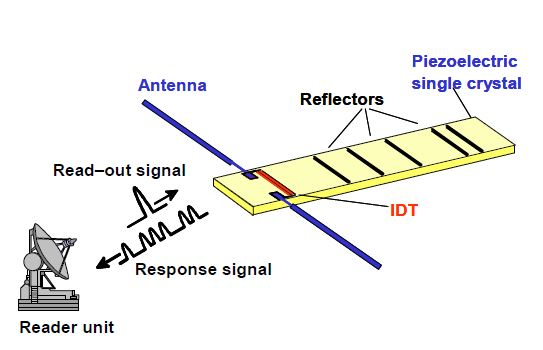
\includegraphics[width=0.375\textwidth]{SAWdelay.JPG}
\caption{Schematic of the operating principle of a SAW-based radio-link temperature measurement system. \cite{SAW1}\label{fig:SAWbasic}}
\end{figure}

Having said that, it is also known to use wavelength as the sensing parameter \cite{SAWapps}. The SAW can only be stimulated when the incoming wavelength matches the period of the IDT finger spacing. Thus by emitting a chirp signal it is possible to determine the IDT period, which could be designed to sense strain.

Liu Bo \textit{et al.} \cite{SAWapps} discusses the significance of temperature and mass loading on the wave speed. Temperature ($T$) directly influences the phase velocity and this effect is usually referred to as Temperature Coefficient of Frequency or TCF. For a constant wavelength ($\lambda$) the wave speed ($v$) will vary as the frequency ($f_0$) varies. The frequency variation is described by the following equation

\begin{equation}
TCF = \frac{1}{f_0}\frac{\textrm{d}f_0}{\textrm{d}T} = \frac{1}{v}\frac{\textrm{d}v}{\textrm{d}T}- \frac{1}{\lambda}\frac{\textrm{d}\lambda}{\textrm{d}T}\textrm{.}
\end{equation}


Many other factors which affect the propagation velocity are based on the mass loading of the piezoelectric substrate. For example chemical sensing can be accomplished by depositing suitable layer on top the substrate that reacts with the chemical of interest, thus changing the mass loading conditions. According to Sauerbrey equation \cite{mass} mass loading has a linear effect on the frequency change

\begin{equation}
\frac{\Delta f}{f_0} \simeq -\frac{\rho _m t_m}{\rho _0 t_0} = -\frac{\Delta m}{m_0}\textrm{,}
\end{equation}

where $m_0$ is the equivalent mass of the resonant part of the device, $\rho _m$ and $t_m$ are the density and thickness of the mass on the SAW propagating path, and $\rho _0$ and $t_0$ are the density and thickness of the unloaded resonator respectively \cite{SAWapps}.

In terms of applications there are countless publications reporting the use of SAW sensors for temperature \cite{sawtemp1, sawtemp2}, pressure \cite{sawtemp2, sawpres1, sawpres2, sawpres3}, humidity \cite{sawhum}, gas \cite{sawgas}, chemical compounds \cite{sawchem1, sawchem2} and bio-agents \cite{sawbio1, sawbio2} measuring. Further details presented in the aforementioned papers won't be discussed here as the main principle of operation has been presented.


\subsection{Relaxation Oscillator}

Patterson \textit{et al.} in their paper \cite{relax} discuss the use of passive wireless sensor for what they call chem-bio agents. First of all in their research they advocate the use of inductive coupling over RF. The reason for that is more efficient power transfer, however they rightly noticed that it comes at a cost of greatly decreased range. They report peak power transfer at 1.5 cm.

The research group proposed to first convert the incident AC signal into DC using full bridge rectifier. This DC is then used to drive a tunable oscillator. The schematic of the circuit is shown in Figure \ref{fig:circuit}.

\begin{figure}[h]
\centering
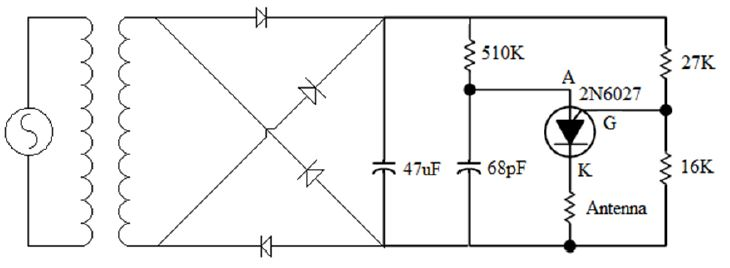
\includegraphics[width=0.5\textwidth]{relax.JPG}
\caption{Schematic diagram of the sensor based on relaxation oscillator \cite{relax}\label{fig:circuit}}
\end{figure}

The circuit works by charging the capacitor connected to the anode to a threshold voltage determined by the bias resistor pair on the gate side. The input resistor limits the charge time, but it also limits valley current to cut off the the unijunction transistor during the discharge segment of operation. When the voltage across the capacitor slightly exceeds that of the bias on the gate, the unijunction transistor turns on and discharges the capacitive energy through the cathode. Since the the input charge resistor limits the amount of current that can flow once the capacitor discharges, the unijunction transistor shuts off and the cycles starts over again. The reason the transistor shuts off is that it requires a minimum current to flow through it to maintain the on state. This is referred to as valley current.

This circuit has the ability to act as a sensor only when either bias or the anode capacitance vary. In the paper they proposed to introduce a variable capacitor in parallel with a fixed value one. That way they were able to alter the frequency of the output signal with variation in capacitance. The output frequency was recorded to be around 40 kHz which makes it applicable for RF applications, however it would require a large antenna.

\subsection{Metamaterial Structures}

Metamaterials are artificial materials engineered to exhibit properties which are not readily found in nature. Generally isotropic dielectrics at a given frequency have positive permittivity and permeability, thus resulting in a real and positive refractive index. However, metamaterials exhibit negative permittivity and permeability and thus have a real but negative refractive index. For completion, we can also distinguish two other sets of material, i.e. plasma or metals at optical frequencies and ferrites. The former has negative permittivity and positive permeability, whereas in the latter the signs are reversed. Either way, the refractive index ends up being negative and imaginary. In those cases there is no propagation and we only observe an evanescent wave.

There are no known naturally existing materials that exhibit meta properties. However, structures that behave as such have been successfully engineered. One such example is a split ring resonator or SRR shown in Figure \ref{fig:srr}. Note that both of the squares have gaps - larger one at the top and the smaller one at the bottom.

\begin{figure}[h]
\centering
\begin{subfigure}{.5\textwidth}
  \centering
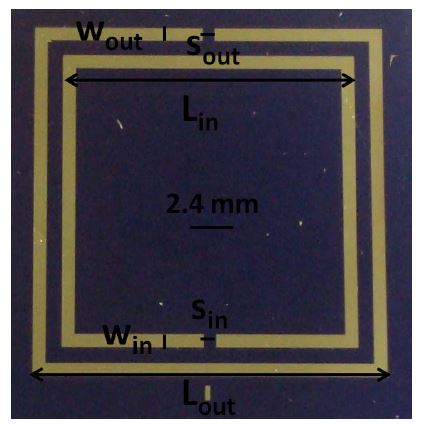
\includegraphics[width=0.75\textwidth]{srr.JPG}
\caption{Traditional split ring resonator structure.\label{fig:srr}}
\end{subfigure}%
\begin{subfigure}{.5\textwidth}
  \centering
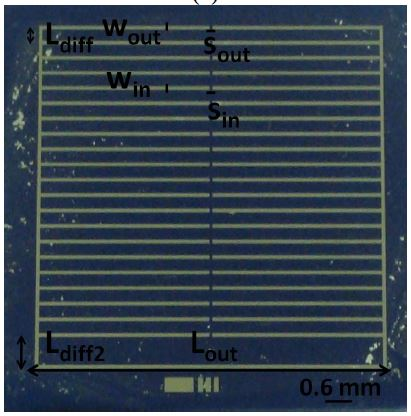
\includegraphics[width=0.75\textwidth]{nested.JPG}
\caption{Nested split ring resonator structure.\label{fig:nested}}
\end{subfigure}
\caption{Plan view pictures of two SRR structures. \cite{srr}}
\end{figure}

These types of structures are usually very narrowband. Most of the time they behave as right-handed materials.

Melik \textit{et al.} \cite{srr} proposed using metamaterial structure for strain sensing in medical application space. The advocate using it over traditional materials as metamaterials tend to have lower resonant frequency, which was of advantage to them since higher frequencies would be absorbed by soft tissue. Moreover, these artificial materials exhibit much higher Q-factors compared to standard spiral structures. This enables tracking of the resonant frequency more comfortably. Thirdly, linearity is much easier achieved when compared to traditional spiral structures, thus allowing to infer the measured quantity directly form the slope. Final point wraps back to the first one in that metamaterials can support much larger wavelengths for the same size, hence their size can be greatly reduced.

The research group then used the splits in the rings as the means of measuring strain. As the gap size varies the resonant frequency of the structure varies with it, and hence it is possible to determine the magnitude of stress or strain.

In the same paper, they propose to go a step forward and introduce a nested metamaterial structure, which is shown in Figure \ref{fig:nested}. This structure is reported to have further increased the Q-factor, and sensitivity. At the same time it allowed them to further decrease the operating frequency by some 23 MHz from 529.8 MHz to 506.2 MHz.

\section{Potential Technologies}

\subsection{Sensing Based On Impedance Mismatch}

By performing the scattering or S-parameter analysis of any device we can determine key values such as $S_{11}$ or $S_{21}$, which represent the return and insertion losses respectively. For a lossless device the reflected power and transmitted power should add up to the original signal power.

For a perfectly matched, i.e. impedance complex conjugate matched, systems the values of the S-parameters are $S_{11} = -\infty$ dB and $S_{21} = 0$ dB. However, it is virtually impossible to be able to always perfectly match devices such as a 50 $\Omega$ antenna with the rest of the circuit. As such there will always be some portion of the input signal that is going to be reflected. The magnitude of the backscattered signal will depend on how poorly the systems are matched. Thus, by exploiting this idea it is possible to make a circuit whose impedance will vary relative to the antenna, or vice-versa.

\subsection{Sensitive Slow Wave Structures}

Similar to surface acoustic waves, it would be possible to slow down electromagnetic waves and employ similar techniques to those of SAW. The key differences between this solution and SAW are as follow; firstly, surface acoustic wave is a mechanical, elastic wave whereas slow wave structures are still based on electromagnetic propagation. Secondly, the reported slow down factor in SAW was in the excess of 1000 over the free space counterpart. In slow wave structures we should not expect as high slowing factors. It is reasonable to assume less than a 100 fold decrease in group velocity.

We can distinguish high-$\kappa$ and low-$\kappa$ dielectrics. These are essentially materials with high and low relative permittivity. An example of a low-$\kappa$ dielectric is silicon dioxide SiO$_2$, which has a dielectric constant of just 3.9. This means that an electromagnetic wave will only slow down by a factor of around 2. A high-$\kappa$ materials include compounds such as strontium titanate which is reported to have relative permittivity of 186 \cite{strtit}, which corresponds to slow down factor of around 13.5. It has also been reported \cite{bst} that under special circumstance barium strontium titanate (BST) films can achieve relative permittivity of as high as 1200, which represents a slow down of 34.5.

It is therefore clear that material itself is not sufficient in providing the required slow down for the EM waves. Special structures should be employed such as metal-insulator-semiconductor (MIS) \cite{phd} or MIS-ferrite (MISF). These structures allow to separate electric and magnetic fields, thus providing virtually any required slow-downs. It is in fact theoretically possible to stop the wave altogether if such structure operates at its resonant frequency \cite{misf}.

Having slowed down the wave such that any time delays are now possible to measure over shorter distances, it is now only a matter of somehow modulating the wave as it propagates through the structure or as in the case of SAW - reflecting it. Reflection seems a more achievable task. Hence the structure would be required to stretch and compress under various conditions such as temperature or pressure change.

\section{Conclusion}

In this review paper several existing technologies have been presented. We can clearly distinguish six or seven categories of passive wireless sensors. Firstly, there are those which explicitly employ an LC(R)-resonant tank, wherein either an inductor or a capacitor plays the role of tunable element sensitive to environmental changes.

Secondly, there are resonant surfaces, which due to their geometry support only specific modes and frequencies. Those modes can be excited using a chirp signal and thus if the geometry of those surfaces varies, the information can be decoded from the frequency of the return signal.

Separate to those, we have metamaterial structures. These are the special type of devices, which behave differently than it might be expected. At certain frequencies metamaterial structures exhibit properties which are not found in nature such as negative permittivity and permeability. Though the operational principle is similar to those of e.g. cavity resonator, the fact that these are metamaterials gives them extra advantages such as higher quality factor, lower resonant frequencies and increased linearity.

As mentioned we could also carve out separate group of resonant structures such as evanescent-mode cavity resonator. Its principle of operation is very similar to that of LC-tank, however the passive elements aren't explicitly present, rather they arise as a form of parasitic behaviour.

Fifthly, intermodulation communication principle has been revised. This method tackles the problem of passive wireless sensing rather differently to the resonant approaches. By illuminating the sensor with two nearby frequencies, some electrically non-linear element or a MEMS is used to mix them together. The difference frequency is then extracted and used to stimulate a resonant circuit. Depending on the response of the circuit the voltage generated at the difference frequency will vary. That signal then mixes back with the incident waveforms and is reflected back to the interrogator.

As niche group we can identify relaxation oscillators as a form of PSW. The circuits oscillation frequency is determined by the measurand. This particular method is not suitable for RF, as the resultant frequencies are too low for efficient broadcasting and preservation of good SNR.

Finally, we have surface acoustic wave passive wireless sensors. These sensors differ from others in that they utilise mechanic and elastic waves to relay information between antennas. SAW devices act as sensors, because they are able to slow down an electromagnetic wave thousands of times and introduce reflections, whose time-spacing is environment-dependent.

Depending on an application and application space various methods might be of benefit. As such optimal solution must be found individually for every problem.

\bibliography{mybib1}{}
\bibliographystyle{unsrt}

\end{document}